
\begin{frame}
\frametitle{Laufzeitanalyse}
\framesubtitle{Fall 2}

\begin{enumerate}
	\item[1.] Improved-Graph $G'$ berechnen
\end{enumerate}
\ \\
\begin{itemize} %TODO Umformatieren
	\item Knoten durchzählen $(v_1, v_2, \dots, v_n)$
	\item Queue $Q$ mit Tripeln der Form $((v,w),x)$ oder $((v,w),-)$ mit $v,w,x \in V$
	\item Array $S$ mit Liste $S[v_i]$ die für $v_i$ Paare von Knoten enthält
	\item $\forall (v_i, v_j) \in E$ mit $i < j \rightarrow ((v_i, v_j), -)$ in $Q$ einstapeln
	\item $\forall v \in V$ mit deg($v$) $\leq k \rightarrow$ Alle Nachbarpaare $v_i, v_j \in N_G(v)$ durch $((v_i, v_j),v)$ in $Q$ einstapeln
\end{itemize}
$\vdots$

\end{frame}


\begin{frame}
\frametitle{Laufzeit}
\framesubtitle{Visualisierung}


\end{frame}


\begin{frame}
\frametitle{Laufzeitanalyse}
\framesubtitle{Fall 2}

$\vdots$
\begin{itemize}
	\item $Q$ zweimal bucket-sortieren, erst nach dem ersten, dann nach dem zweiten Knoten im Tupel \\
	$\rightarrow$ Alle Tripel $((v_i, v_j),v)$ mit gleichem $i,j$ sind hintereinander \\
	$\Rightarrow$ Es kann schnell geprüft werden welche Paare $k+1$ gemeinsame Nachbarn haben
	\item Sind min. $k+1$ Einträge $((v_i, v_j), v)$ für ein Paar $v_i, v_j$ in $Q$ untereinander $\Rightarrow (v_i, v_j)$ ist in $G'$
	\item Für jedes obiges Paar $(v_i, v_j)$ und wenn $((v_i, v_j), -) \in Q \rightarrow$ Füge $(v_i, v_j)$ für jedes $((v_i, v_j), v)$ zu $S[v]$ hinzu
\end{itemize}
\ \\
\ \\

$S[v]$ enthält nun alle Kanten von Nachbarn von $v$. Da deg($v$) $\leq k$ ist $S[v]$ durch $k$ beschränkt. \\
Damit kann durch ansehen von $S[v]$ entschieden werden ob $v$ I-simplizial ist.
\end{frame}


\begin{frame}[t]
\begin{figure}[htbp] 
	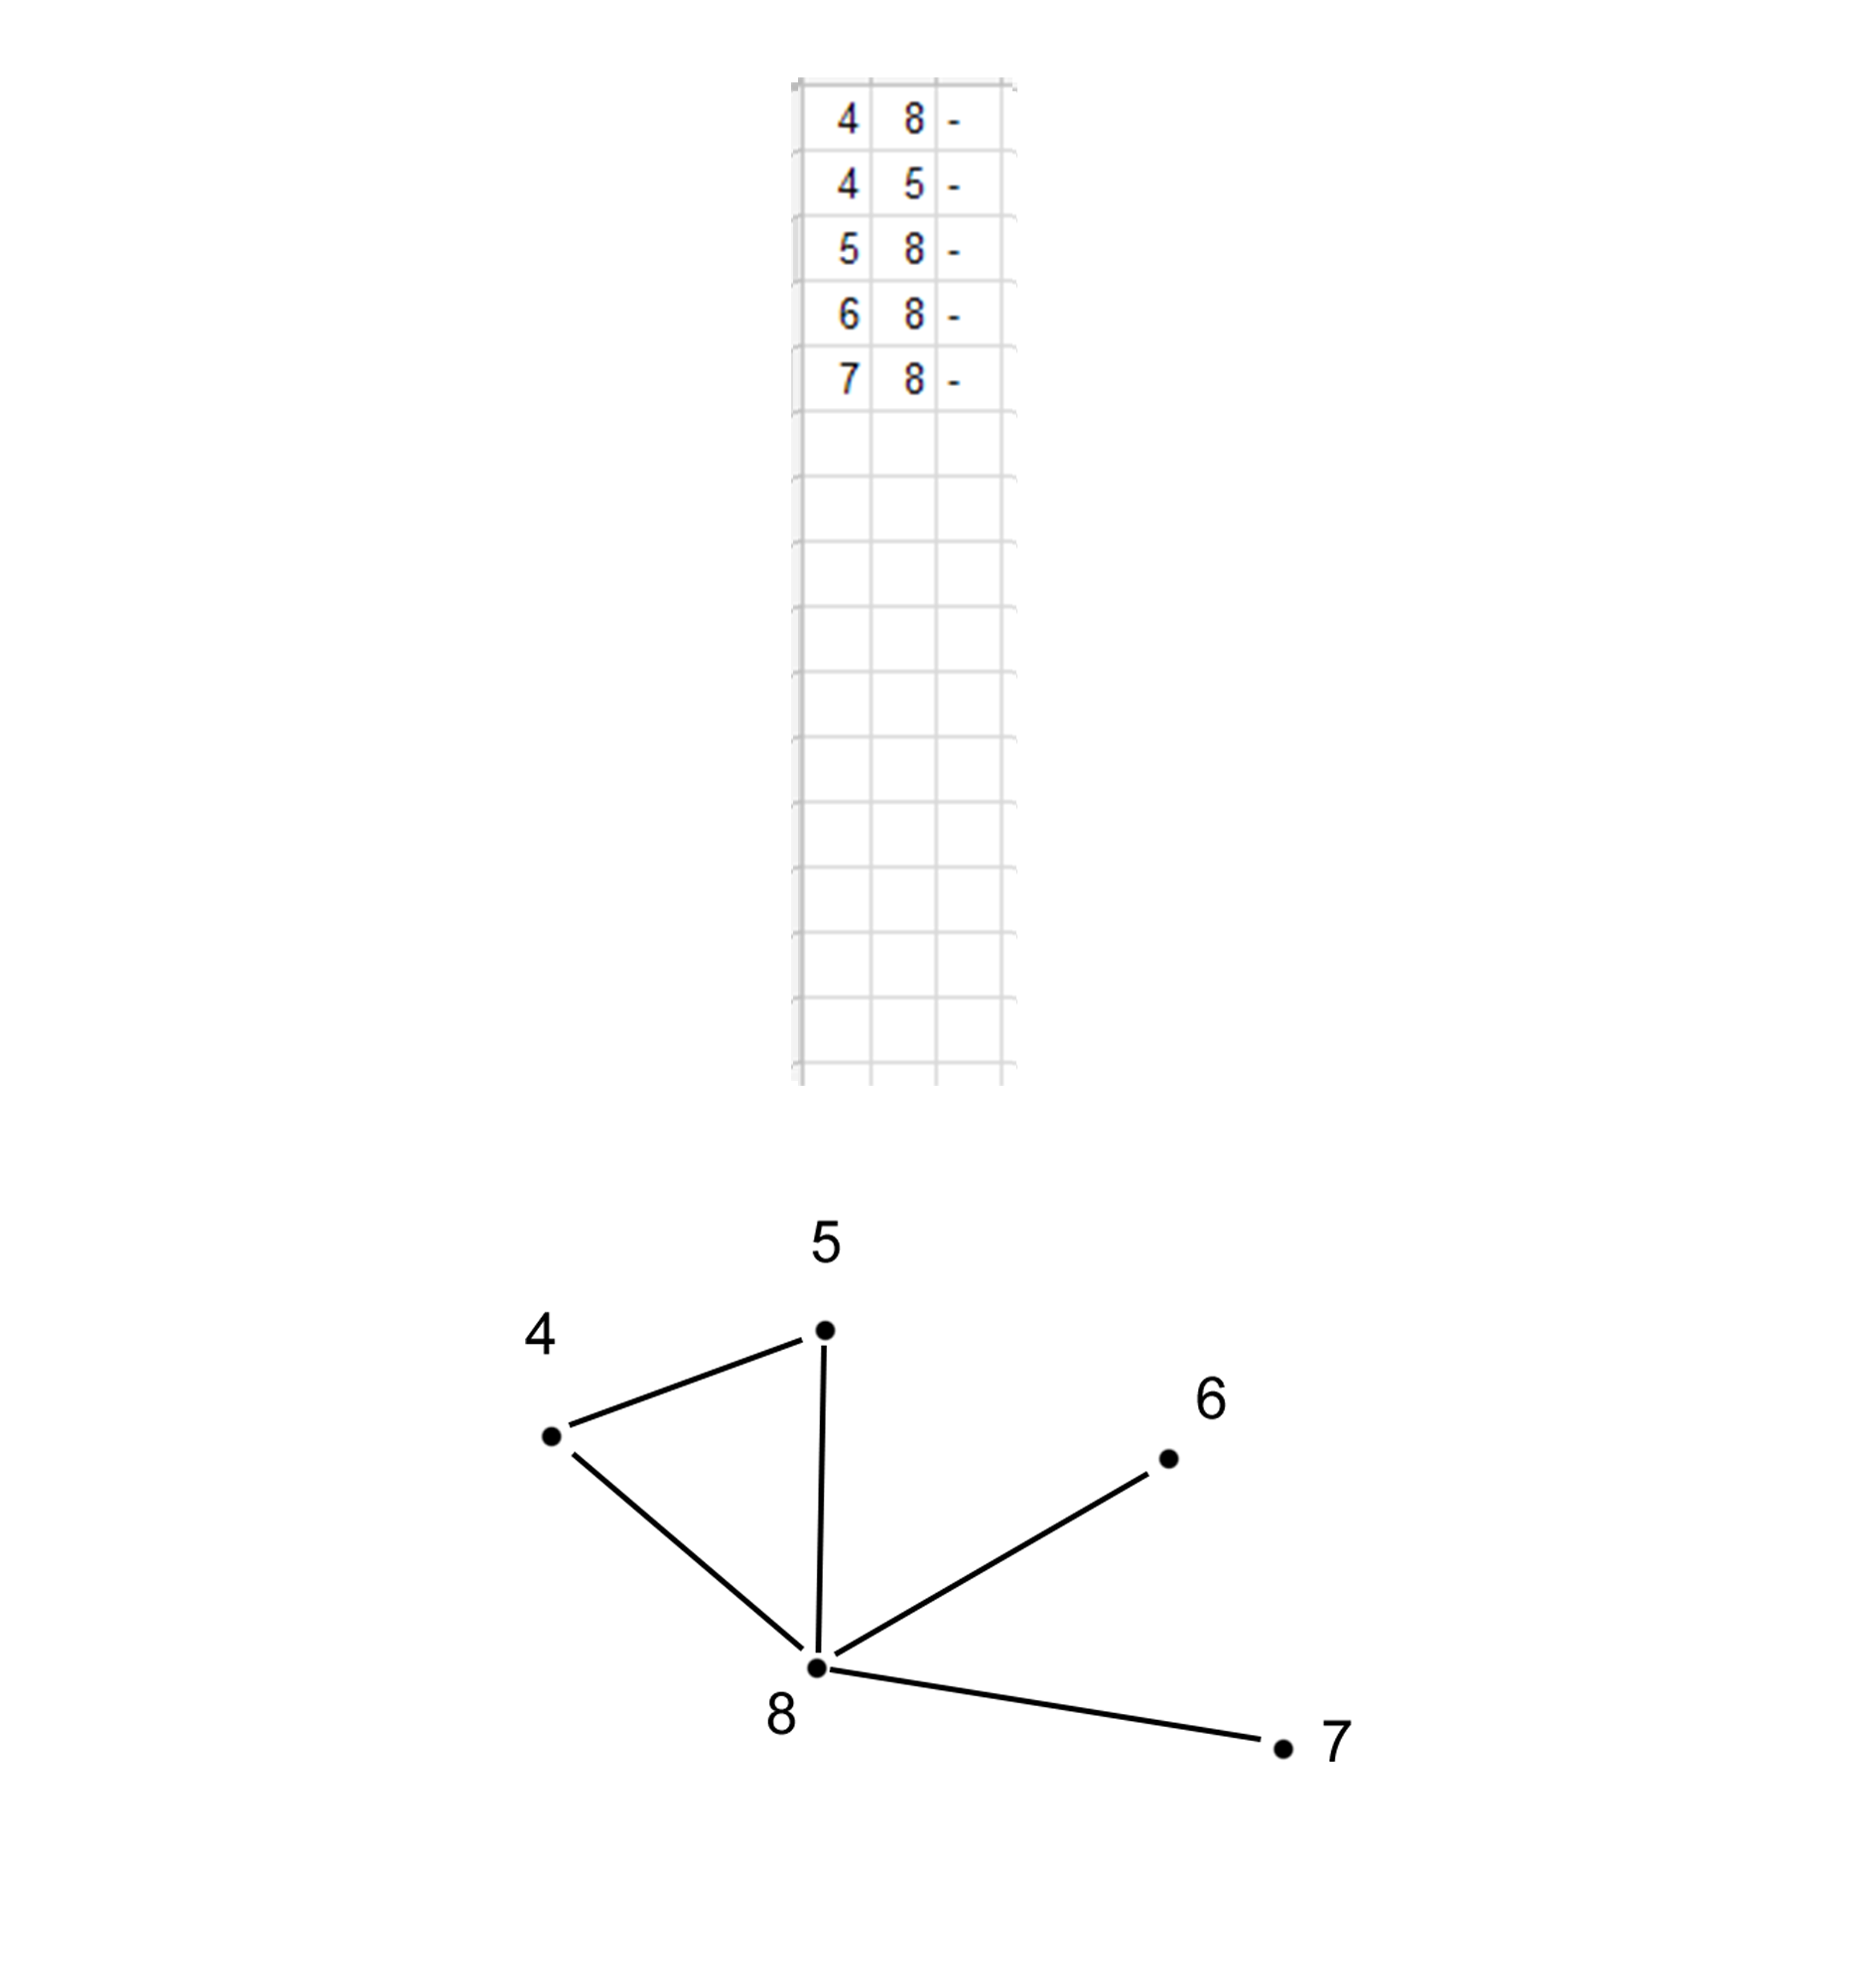
\includegraphics[width=0.7\textwidth]{images/1.png}
	\caption{1}
	\label{fig:Bild1}
\end{figure}
\end{frame}


\begin{frame}[t]
\begin{figure}[htbp] 
	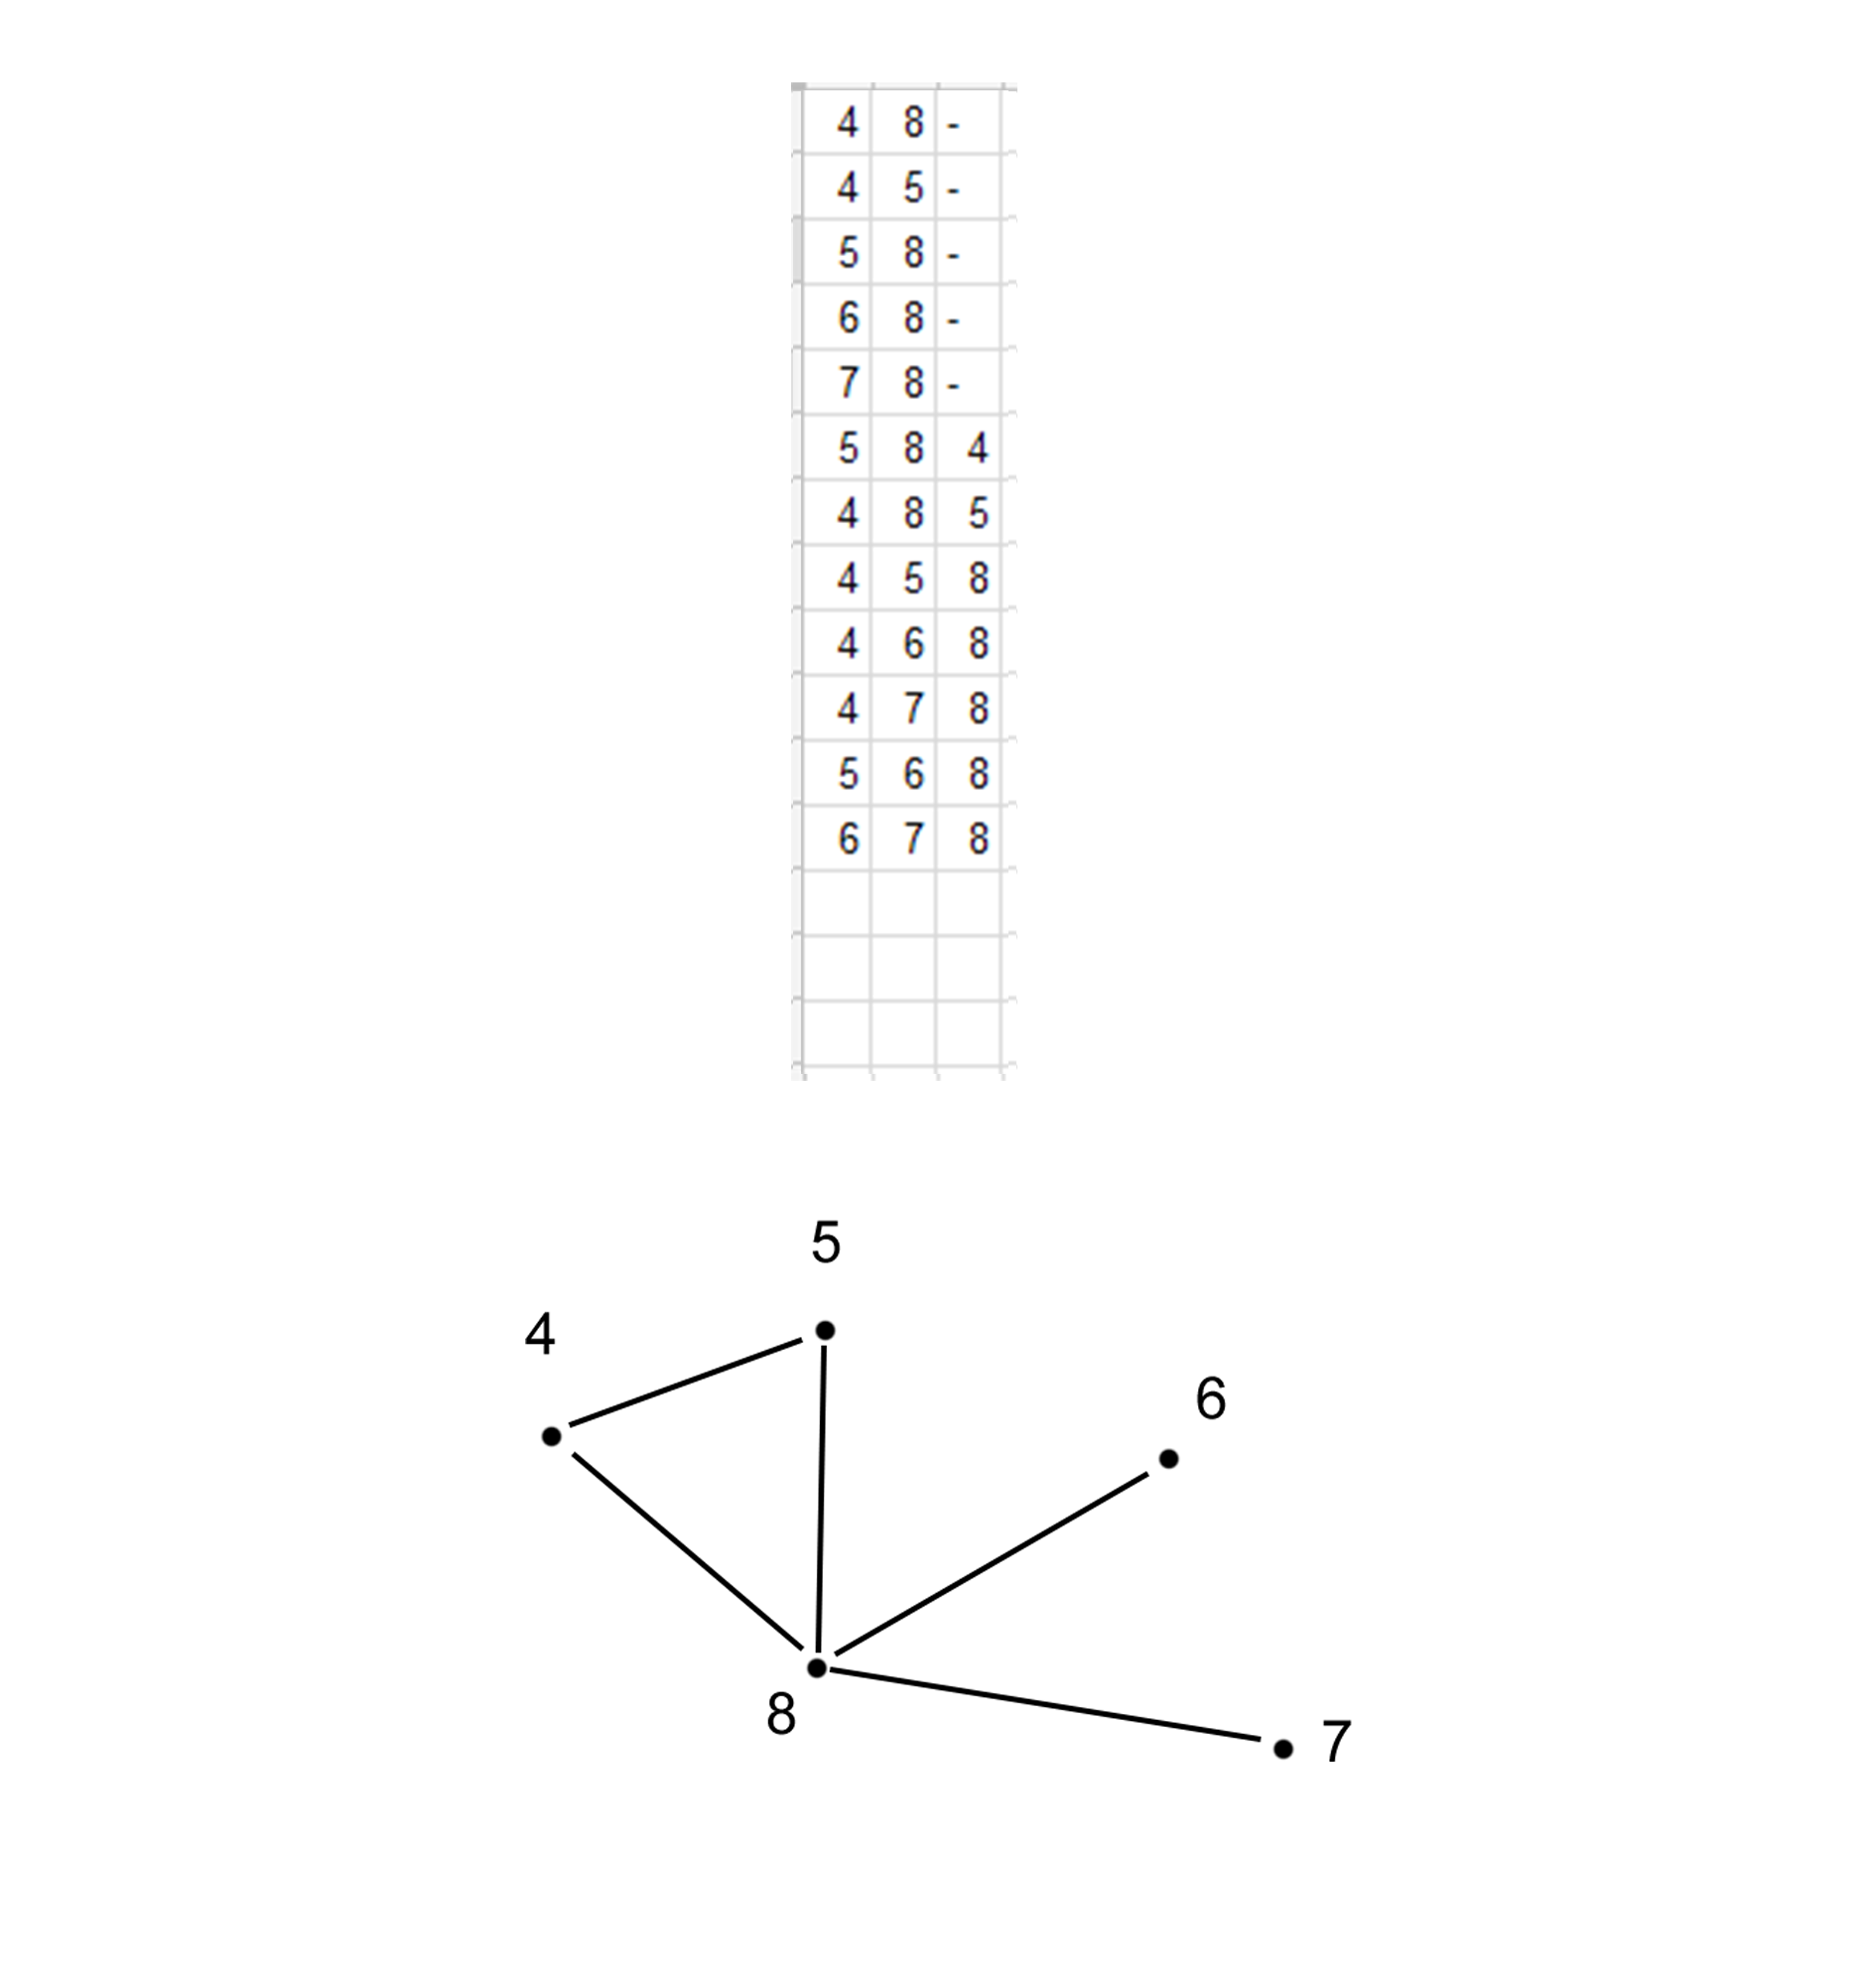
\includegraphics[width=0.7\textwidth]{images/2.png}
	\caption{1}
	\label{fig:Bild1}
\end{figure}
\end{frame}


\begin{frame}[t]
\begin{figure}[htbp] 
	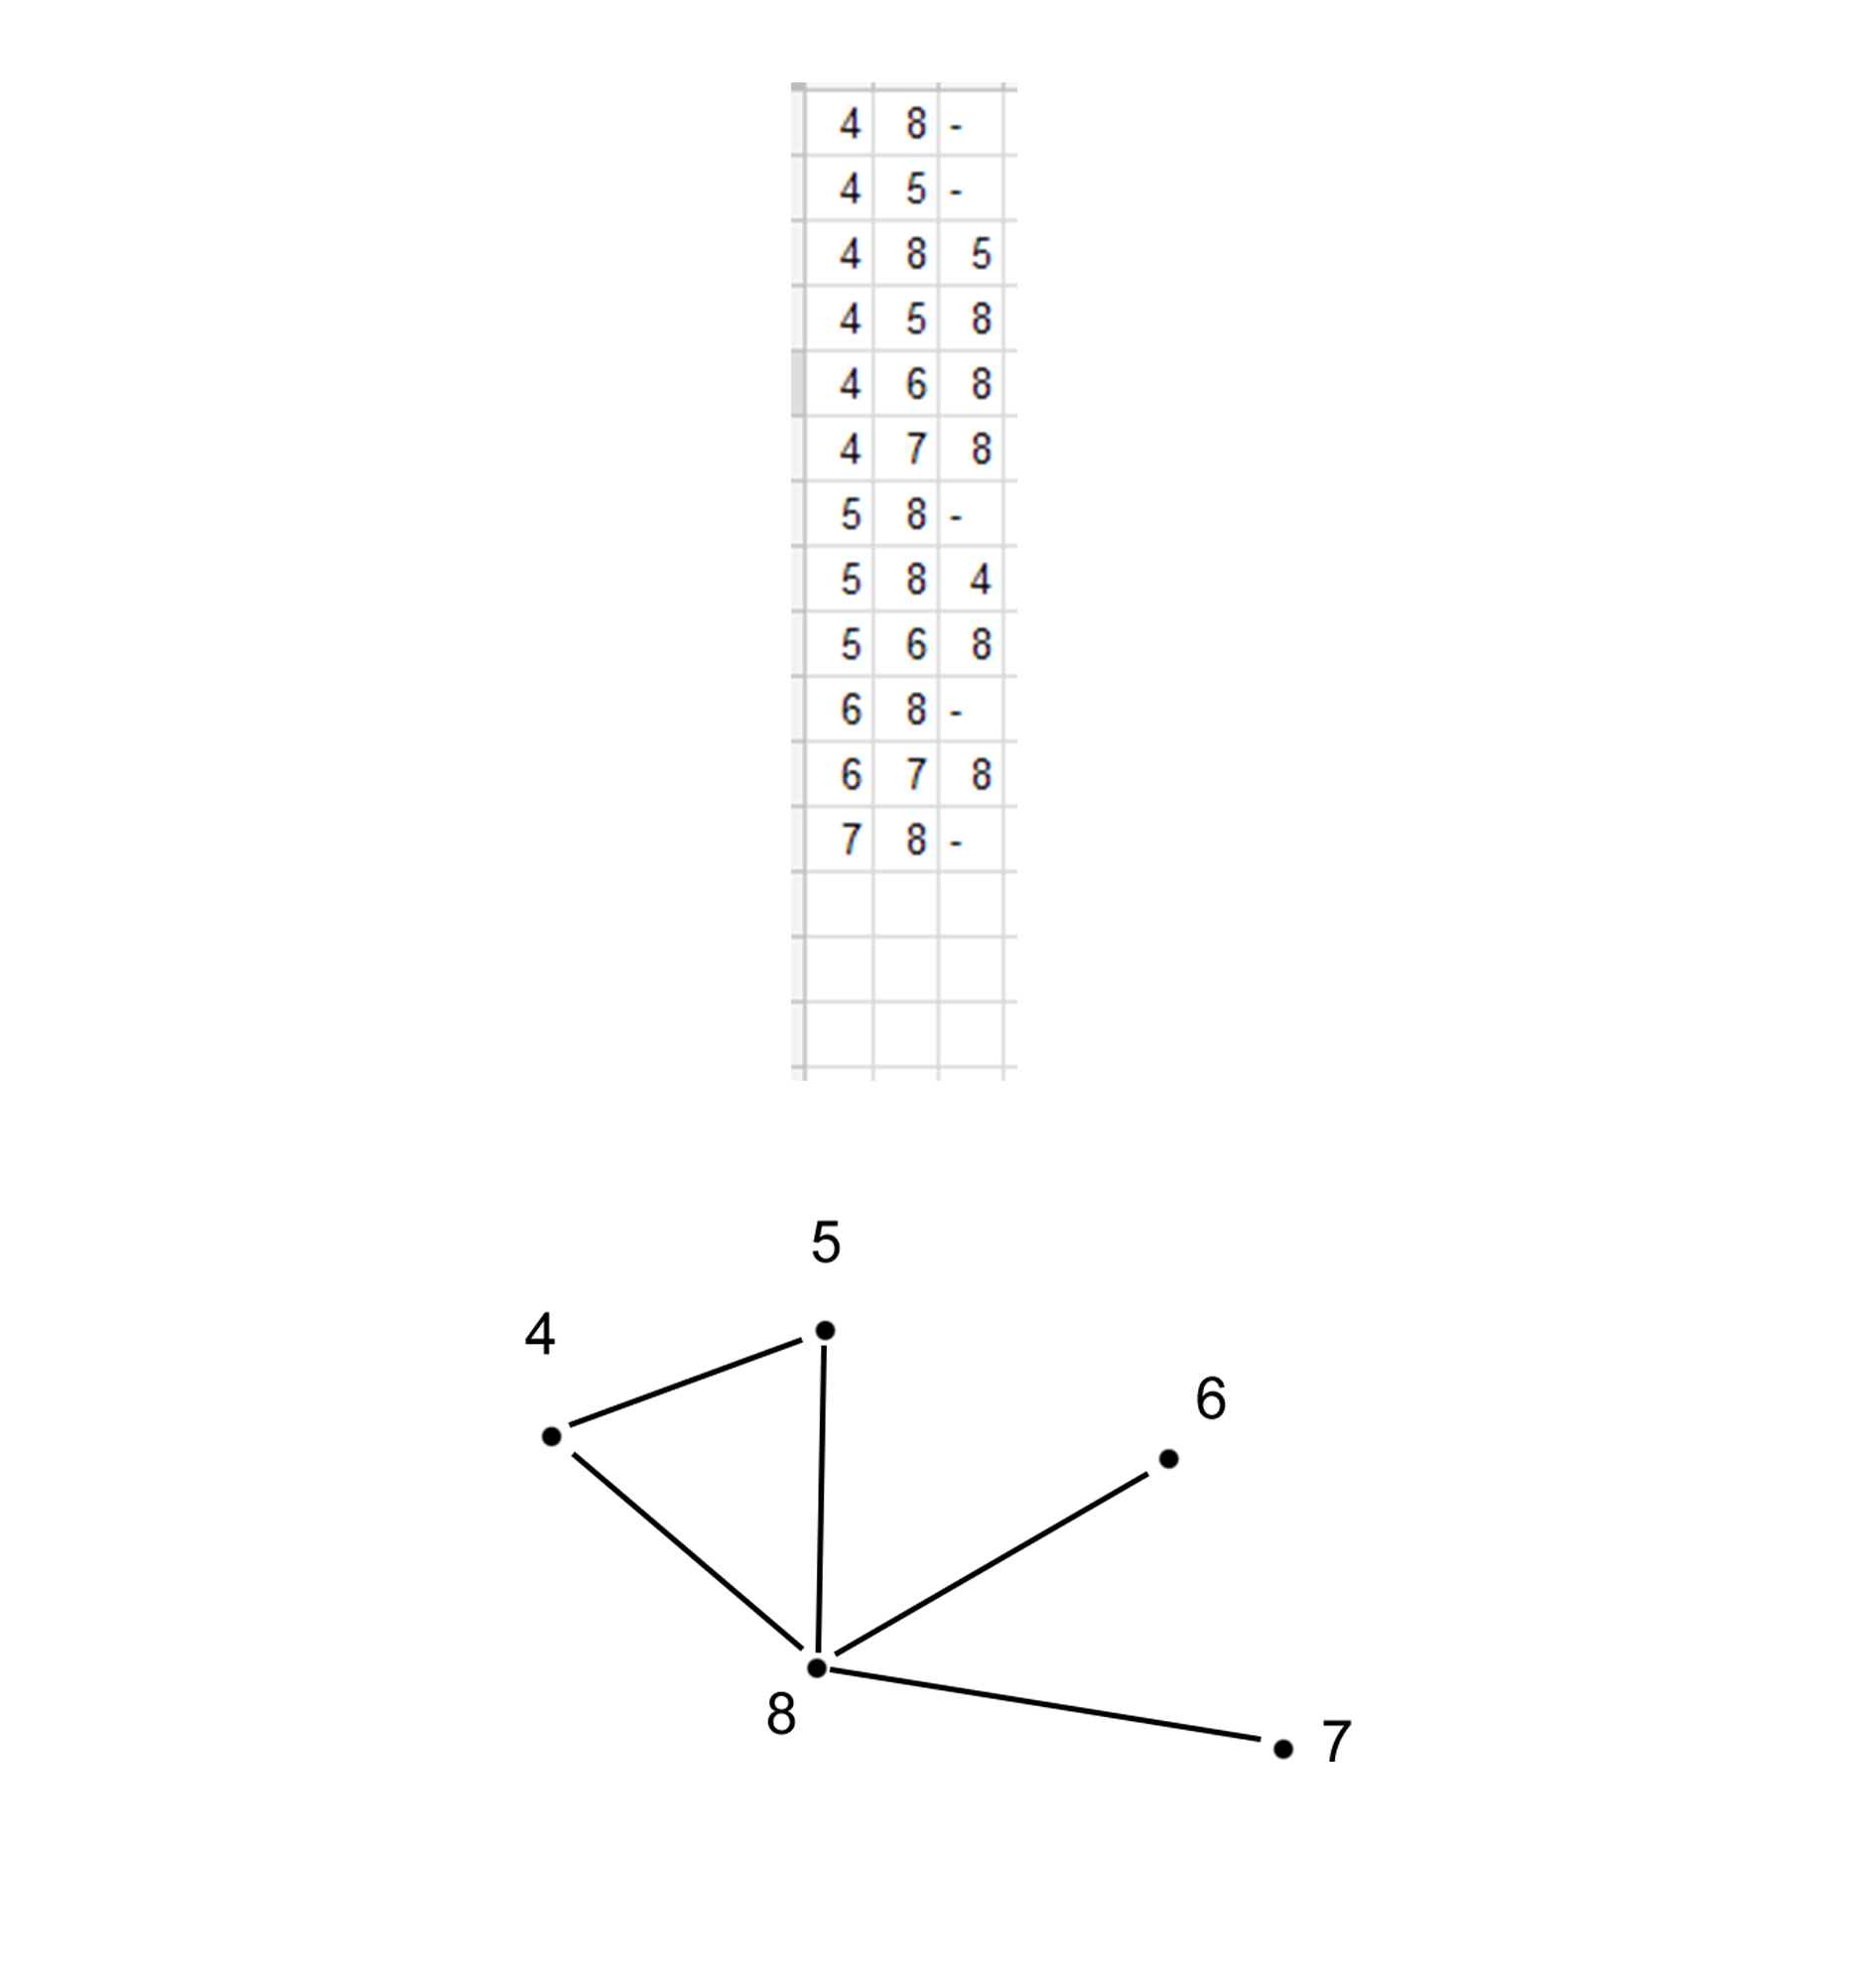
\includegraphics[width=0.7\textwidth]{images/3.png}
	\caption{1}
	\label{fig:Bild1}
\end{figure}
\end{frame}


\begin{frame}[t]
\begin{figure}[htbp] 
	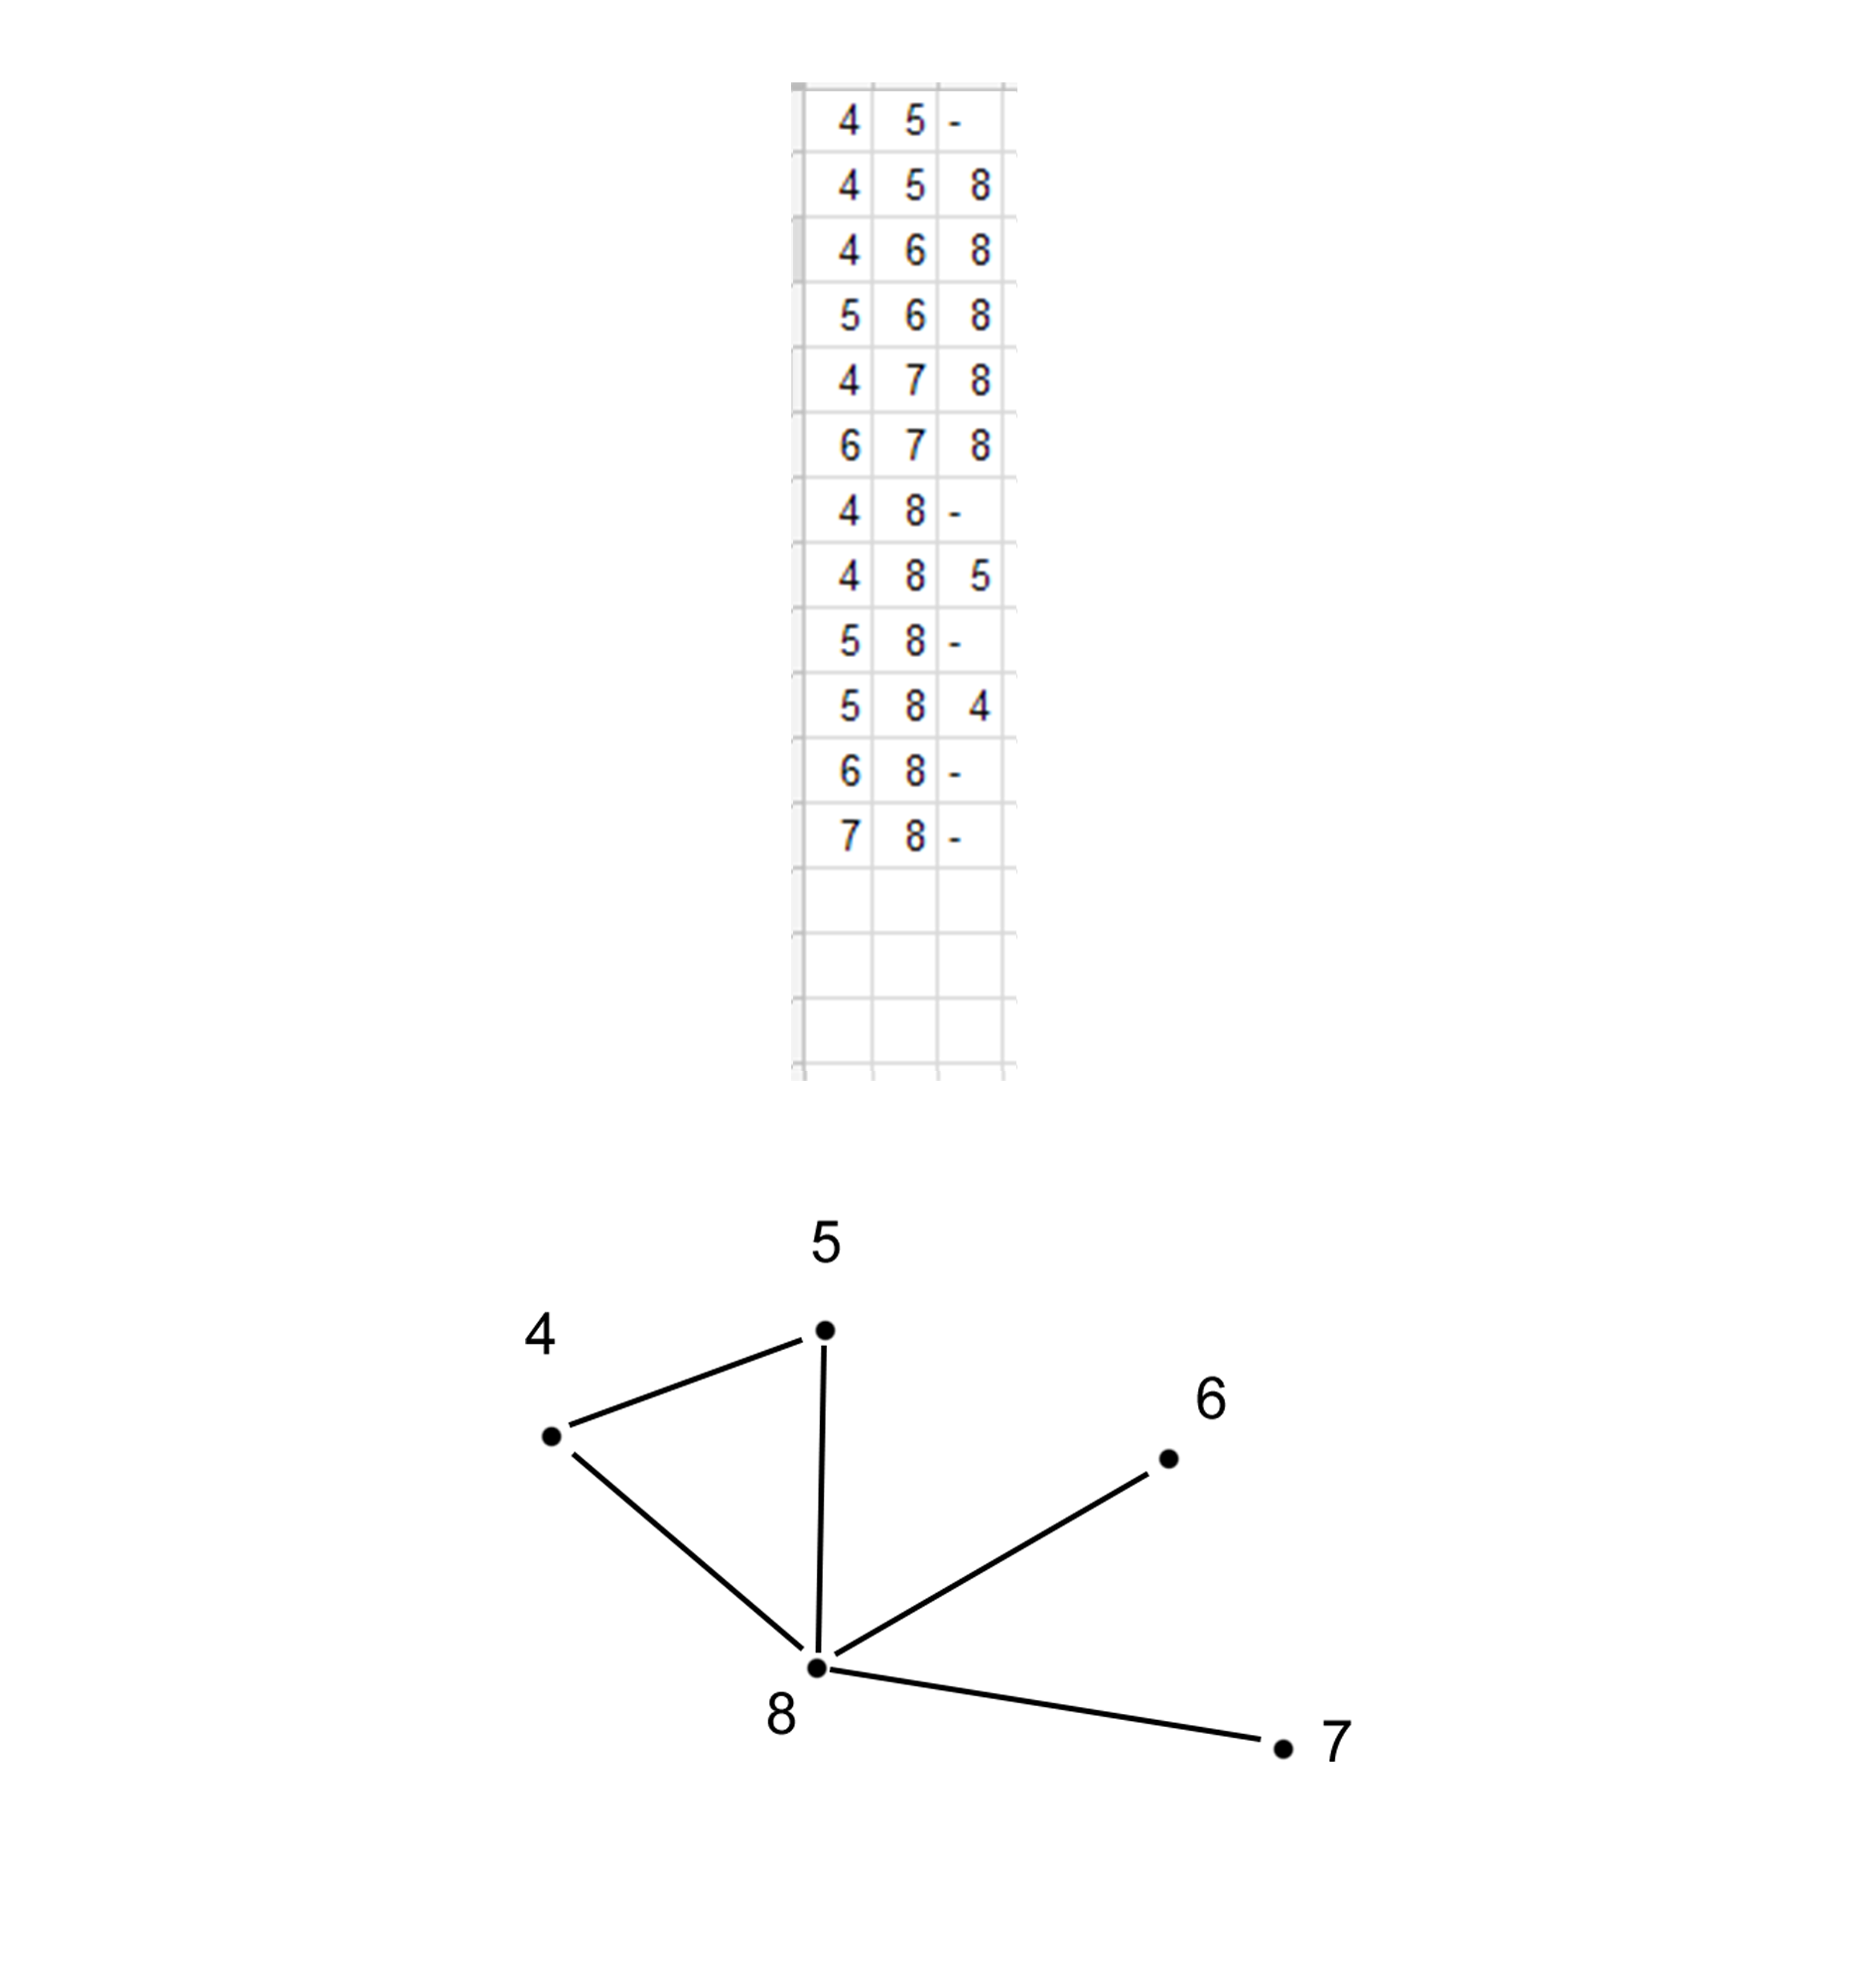
\includegraphics[width=0.7\textwidth]{images/4.png}
	\caption{1}
	\label{fig:Bild1}
\end{figure}
\end{frame}


\begin{frame}
\frametitle{Laufzeitanalyse}
\framesubtitle{Fall 2}

\begin{enumerate}
	\item[2.] Alle I.simp.-Knoten in Menge $SL$ und von $G$ entfernen $\Rightarrow \widehat{G}$ entsteht
\end{enumerate}
\ \\
\ \\
\ \\
\ \\
Durch das Vorgehen von gerade eben können wir die Menge $SL$ in $O(k \cdot n) \in O(n)$ aus $S$ auslesen.

\end{frame}


\begin{frame}
\frametitle{Laufzeitanalyse}
\framesubtitle{Fall 2}

\begin{enumerate}
	\item[3.] Algorithmus rekursiv auf $\widehat{G}$ ausführen
\end{enumerate}
\ \\
\ \\
\ \\
\ \\
Graph $\widehat{G}$ hat nach Entfernung von $SL$ $(1 - c_2) \cdot |V|$ Knoten. \\
\ \\
Wie in Fall 1 sind alle rekursiven Aufrufe in $O(n)$ möglich. \\

\end{frame}


\begin{frame}
\frametitle{Laufzeitanalyse}
\framesubtitle{Fall 2}

\begin{enumerate}
	\item[4.] Füge $SL$ wieder in die Zerteilung $(Y,T)$ ein
\end{enumerate}
\ \\
\ \\
\begin{enumerate}
	\item $\forall v \in SL$: Finde ein $Y_{i_v} \in Y$ in dem alle Nachbarn von $v$ sind ($N_G(v) \subseteq Y_{i_v}$)
	\item Füge $Y_{j_v} = \{ \{v\} \cup N_G(v) \}$ zu $Y$ hinzu und mache es adjazent zu $Y_{i_v}$ \\
	$\Rightarrow$ Baumzerteilung von $G$ mit Baumweite max. $k$
\end{enumerate}
\ \\
$Y_{i_v}$ existiert für jedes $v$, da I.simp.-Knoten in $G$ nicht adjazent sind und $N_G(v)$ eine Clique formt. \\
\textcolor{cyan}{LEMMA 2.1.i)}: "$(X,T)$ Zerteilung von $G$ und $W \subseteq V$ formt Clique in $G \Rightarrow \exists i \in I: W \subseteq X_i$"
\end{frame}

\begin{frame}
\frametitle{Laufzeitanalyse}
\framesubtitle{Fall 2}

\begin{enumerate}
	\item[4.] Füge $SL$ wieder in die Zerteilung $(Y,T)$ ein
\end{enumerate}
\ \\
\ \\

\begin{itemize}
	\item $\forall l \leq k$: Nimm Queue $Q_l$ wo alle Paare $((v_{i_1}, v_{i_2}, \dots v_{i_l}), i)$ für $v_{i_x} \in Y_i$ und für alle $i \in I, i_1 < i_2 \dots i_l$ hinzugefügt werden
	\item Füge zu jedem $Q_l$ noch alle Paare $((v_{i_1}, v_{i_2}, \dots v_{i_l}), v)$ wo $v$ I-simp. ist und $N_G(v) = \{ (v_{i_1}, v_{i_2}, \dots v_{i_l} | i_1 < i_2 \dots i_l \}$
	\item Sortiere jedes $Q_l$ $l$-mal, einmal für jedes $v_{i_x}$ im Tupel. Es entsteht wieder eine Sortierung der $v_i$
	\item Für jedes Tupel $((\dots), v)$ kann nun schnell das Tupel $((\dots), i)$ gefunden werden
	\item Mache den neuen Knoten $j_v$ mit $X_{i_j} \{ v \} \cup N_G(v)$ zu dem $i$ adjazent und füge ihn zu $Y$ hinzu
\end{itemize}
\ \\
Diese Schritte sind alle zusammen in $O(n)$ ausführbar.
\end{frame}
